
\chapter{Experimental methods\label{chap:Experimental-Methods} }

\addcontentsline{lof}{chapter}{Experimental methods\lofpost}  
%\addcontentsline{lot}{chapter}{Experimental methods\lofpost}          
  
\singlespacing
\epigraph{ 
If I knew what I was doing, it wouldn't be called research.}    
{Albert Einstein\\
See \citet{hawken2010natural}}   
\doublespacing\noindent  \noindent\lettrine{T}{he} design of the superconducting three-level
atom and readout cavity is presented in Sec.~\ref{sec:circuit-design}.
It was optimized subject to the constrains of the experiment (Hamiltonian
and dissipative) with the energy-participation ratio (EPR) approach,
presented in Sec.~\ref{subsec:Energy-participation-ratio}. The methodology
of the finite-element numerical simulations employed to engineer the
electromagnetic (EM) properties of the distributed circuit is presented
in Secs.~\ref{subsec:Calculation-of-EPR} and~\ref{subsec:Calculation-of-Hamiltonian}.
Sample fabrication is discussed in Sec.~\ref{sec:Fabrication-of-sample},
while design and assembly of the sample holder are discussed in Sec.~\ref{sec:Sample-holder-materials}.
Particular attention is paid to material selection, a care continued
in Sec.~\ref{sec:Cryogenic-setup}, where aspects of the cryogenic
setup of the experiment are discussed, including sample thermalization,
surface preparation, light-tightness, and magnetic shielding. The
microwave setup of the experiment is discussed in Sec.~\ref{sec:Microwave-setup}.
For further information on experimental methods employed in circuit
quantum electrodynamics (cQED) experiments see Refs.~\citet{Geerlings2013,Reed2013,Reagor2016,Brecht2017-Thesis}.

\section{Sample design \label{sec:circuit-design}}

\paragraph{Overview. }

The superconducting artificial atom presented in Sec.~\ref{sec:Principle-of-the},
see Fig.~\ref{fig:Sample-design-assembly}a, consists of two coupled
transmon qubits \citep{Koch2007,Schreier2008-transmon,Paik2011} fabricated
on a 2.9~mm-by-7~mm double-side-polished c-plane sapphire wafer
with the Al/Al$\text{O}_{\text{x}}$/Al bridge-free electron-beam
lithography technique \citep{Lecocq2011-bridge-free,Rigetti2009};
for fabrication methodology, see Sec.~\ref{sec:Fabrication-of-sample}.
The first transmon (B) is aligned with the electric field of the fundamental
$\mathrm{TE}_{\mathrm{101}}$ mode of the aluminum rectangular cavity
(alloy 6061; dimensions: 5.08~mm by 35.5~mm by 17.8~mm), while
the second transmon (D) is oriented perpendicular to the first and
positioned $170\,\mathrm{\mu m}$ adjacent to it, see Fig.~\ref{fig:Sample-design-assembly}b.
The inductance of the Josephson junction of each transmon (nominally,
9~nH for both B and D), the placement and dimensions of each transmon,
and the geometry of the cavity were designed and optimized using finite-element
electromagnetic analysis and the energy-participation-ratio (EPR)
method\footnote{Z.K. Minev \emph{et al.}, in preparation.}, as discussed
in Sec.~\ref{subsec:Energy-participation-ratio}. 

\begin{figure}
\centering{}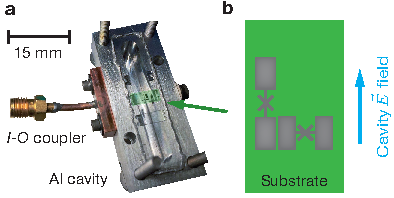
\includegraphics[scale=1.4]{methods/sample-assembly}
\caption[Sample and chip layout]{\textbf{Sample and chip layout.\label{fig:Sample-design-assembly}}
\textbf{a,} Photograph of Darkmon chip ($2.9\times7$~mm, sapphire)
in the aluminum (Al) cavity, which serves as the sample holder, shown
with upper half removed. Green arrow points to location of the chip.
Also visible: input-output (\emph{I-O}\textbf{) }SMA coupler and frequency
tuning screw (right side). \textbf{ b, }Not-to-scale schematic representation
of the Bright (vertical) and Dark (horizontal) transmon qubits. Vertical
blue arrow indicates the orientation of the electric field of the
fundamental ($\mathrm{TE}_{\mathrm{101}}$) cavity mode. }
\end{figure}


\paragraph{Hamiltonian and level diagram.}

Under the rotating-wave approximation and in the low-excitation limit,
see Sec.~\ref{subsec:Calculation-of-Hamiltonian}, the effective
Hamiltonian of the device, consisting of the Dark, Bright, and cavity
modes, is energy conserving, 
\begin{align}
\hat{\overline{H}}/\hbar= & \omega_{{\rm D}}\hat{n}_{\emph{{\rm D}}}+\hbar\omega_{{\rm B}}\hat{n}_{{\rm B}}+\hbar\omega_{{\rm C}}\hat{n}_{{\rm C}}\nonumber \\
 & -\frac{1}{2}\alpha_{{\rm D}}\hat{n}_{\emph{{\rm D}}}\left(\hat{n}_{\emph{{\rm D}}}-\hat{1}\right)-\frac{1}{2}\alpha_{{\rm B}}\hat{n}_{{\rm B}}\left(\hat{n}_{{\rm B}}-\hat{1}\right)\nonumber \\
 & +\chi_{{\rm DB}}\hat{n}_{\emph{{\rm D}}}\hat{n}_{{\rm B}}+\chi_{{\rm DC}}\hat{n}_{\emph{{\rm D}}}\hat{n}_{{\rm C}}+\chi_{{\rm BC}}\hat{n}_{{\rm B}}\hat{n}_{{\rm C}}\,,\label{eq:HDarkmon}
\end{align}
where $\hat{n}_{{\rm D,B,C}}$ are the Dark, Bright, and cavity photon-number
operators, $\alpha_{{\rm D,B}}$ are the Dark and Bright qubit anharmonicities,
also referred to as self-Kerr frequencies, $\chi_{{\rm DB}}$ is the
dispersive cross-Kerr frequency shift between the Dark and Bright
modes, while $\chi_{{\rm DC,BC}}$ are the dispersive shifts between
the cavity and the two transmons. The energy level structure of the
two-transmon composite system is schematically represented in Fig.~\ref{fig:Darkmon-energy-level-diagram}.
When the anharmonicities, $\alpha_{{\rm B}}$ and $\alpha_{{\rm D}},$
are relatively large, typically in the range 100 to 300 MHz, see Table~\ref{tab:system-params}
for device parameters, the level structure becomes sufficiently anharmonic
and we can restrict our attention to the manifold of the four lowest
energy states, $\left\{ \ket{gg},\ket{eg},\ket{ge},\ket{ee}\right\} $,
where the first (second) letter refers to the Dark (Bright) transmon.
When the two qubits are uncoupled, $\chi_{{\rm DB}}=0$, the transitions
among the levels contain degeneracies, and $\ket{ge}$ and $\ket{eg}$
cannot be addressed individually. In the limit where the coupling,
$\chi_{{\rm DB}}$, is large, in practice, on the order of 100 MHz,
the degeneracy is lifted, and the $\ket{ge}$ and $\ket{eg}$ states
become independent, allowing us to further restrict our attention
to the three lowest-lying states. We label $\ket{gg}$ simply as $\G$,
$\ket{eg}$ as $\D$, and $\ket{ge}$ as $\B.$ In reference to the
protected Dark state, $\D$, which is engineered to be decoupled from
the environment and readout cavity, we  nickname the device ``Darkmon.''

\begin{figure}
\centering{}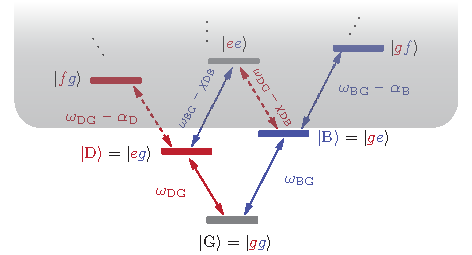
\includegraphics[scale=1.7]{methods/level_diagram}
\caption[Darkmon energy-level diagram]{\textbf{Darkmon energy-level diagram.\label{fig:Darkmon-energy-level-diagram}}
Energy level diagram of the hybridized Dark and Bright transmon qubits.
Red (Blue) color denotes association with the Dark (Bright) transmon,
while grey denotes strong association with both transmons. The strong
non-linear, dispersive interactions in the circuit, self-Kerr ($\alpha_{{\rm B,D}}$)
and cross-Kerr ($\chi_{{\rm DB}}$), allow the lowest-lying three
levels to be isolated, and for the two qubit system to be employed
as a three-level one with a V-shape structure. }
\end{figure}


\paragraph{Unique design constraints. }

In addition to the required large transmon anharmonicity, $\alpha_{{\rm B}}$,
$\alpha_{{\rm D}}$, and cross-Kerr, $\chi_{{\rm DB}},$ frequencies,
a few somewhat unique, decoherence related, constraints were required,
notably, at odds with the large couplings. First, catching and reversing
the quantum jump from $\G$ to $\D$ coherently and with high fidelity
required five orders of magnitude in timescales, see Table~\ref{tab:Summary-of-timescales.},
thus imposing the constraint that the $\D$ level coherences be minimally
at the $100\ \mathrm{\mu s}$ level, both the energy-relaxation and
dephasing times, $T_{1}^{{\rm {\rm D}}},T_{{\rm 2R}}^{{\rm D}}\geq100\,\mathrm{\mu s}$.
The regime of long energy relaxation, $T_{1}^{{\rm {\rm D}}},$ is
accessible with the state-of-the-art Purcell-filtered three-dimensional
(3D) transmon qubits \citep{Paik2011,Wang2015,Dial2016}, but long
quantum coherences, $T_{{\rm 2R}}^{{\rm D}}$, are far more difficult
to achieve, and are generally obtained by decoupling the transmon
qubit from the readout cavity \citep{Gambetta2006-dephasing,Rigetti2012},
thus making a tradeoff between quantum coherence and the ability to
perform a fast readout. In the quantum jumps experiment, this tradeoff
is not permissible, a fast readout of the $\D$ is required simultaneously
with long coherences. 

To maximize the coherence properties of $\D$, we designed the Dark
transmon to be decoupled from all dissipative environments, including
the readout cavity and input-output (I-O) coupler. Removing the coupling
between $\D$ and the cavity is advantageous in three important ways:
it protects $\D$ from i) dephasing due to cavity photon shot noise
\citep{Gambetta2006-dephasing,Wang2019-cav-atten,Wang2018-cav-atten-aps},
ii) energy relaxation through the cavity by means of the Purcell effect
\citep{Gambetta2011-Purcell,Srinivasan2011,Diniz2013,Dumur2015,Novikov2015,Zhang2017,Roy2017-3qubits},
and iii) measurement-induced energy relaxation \citep{Boissonneault2009-Photon-induced-relax,Slichter2016-T1vsNbar},
see Fig.~(\ref{fig:T1-vs-nbar}). Decoupling $\D$ might seem like
a tradeoff at first, since $\D$ can no longer be directly measured
through the cavity. However, the strong coupling between the Dark
transmon and the Bright transmon, together with the special nature
of the V-shape level structure and the $\B$/not-$\B$ dispersive
readout, can be employed to nonetheless achieve a fast and faithful
readout, see Sec.~\ref{subsec:Tomography-of-three-level}. The associated
challenge is that when two transmon qubits are strongly coupled, the
D level needs to remain otherwise isolated and coherent at the same
time that the B level is strongly coupled to the low-quality (low-Q)
cavity. The coupling between $\B$ and the cavity is necessitated
to yield a large dispersive shift, $\chi_{{\rm BC}},$ used to realize
the $\B$/not-$\B$ readout; however, this coupling is accompanied
by a degree of energy relaxation by means of the Purcell effect inherited
by $\B$ \citep{Gambetta2011-Purcell}. The dissipation in $\B$ can
in turn be inherited by the coupled state $\D$, due to the hybridization
between the two transmons, $\chi_{{\rm DB}}$, if the design is not
carefully optimized. 

On a conceptual level, the Darkmon device and the couplings among
the levels can be understood in terms of an effective circuit model,
see Fig.~\ref{fig:Darkmon-circuit}, where each mode is represented
by a single LC oscillator, with the two qubits having the inductors
replaced by non-linear Josephson tunnel junctions. The Dark resonator
is capacitively coupled to the Bright one, which is capacitively coupled
to the readout resonator, which is capacitively coupled to the input-output
transmission line. The Bright and readout resonators can be seen to
act as a two-pole filter shielding the Dark resonator from the dissipative
effect of the transmission line. While the model is conceptually useful
to analyze the qualitative behavior of the circuit, it cannot produce
reliable quantitative results. Instead, engineering the highly asymmetric
set of couplings while isolating the $\D$ level was achieved by means
of an iterative search over the design geometry  with the energy participation
ratio (EPR) approach. In the following, we briefly summarize the methodology. 

\begin{figure}
\centering{}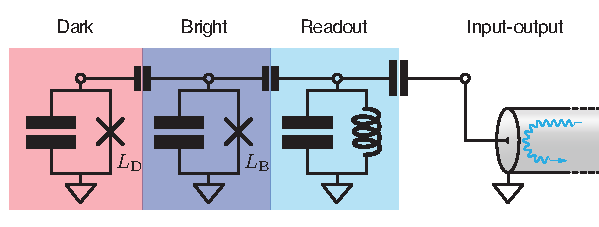
\includegraphics[scale=1.3]{methods/circuit_Darkmon}
\caption[Effective circuit model of Darkmon system]{\textbf{Effective circuit model of Darkmon system.\label{fig:Darkmon-circuit}}
Dark and Bright transmons represented as lumped-element junction-capacitor
circuits, junction denoted by cross, coupled an LC circuit representing
the readout cavity. $L_{\mathrm{D,B}}$ denote the Dark and Bright
Josephson inductances, corresponding to the horizontal and vertical
junctions in Fig.~\ref{fig:Sample-design-assembly}, respectively.}
\end{figure}


\subsection{Energy-participation-ratio (EPR) approach\label{subsec:Energy-participation-ratio}}

The design of distributed circuits with the aim of obtaining a desired
Hamiltonian and set of environmental couplings has attracted a lot
of interest \citep{Nigg2012,Bourassa2012,Solgun2014,Solgun2015,Smith2016},
but a general solution to this inverse problem appears to be out of
reach. Instead, one applies a search algorithm over the direct problem
— a circuit is chosen, the non-linear mixing and dissipation parameters
are calculated, the circuit is modified, and the process is repeated
in search of the target parameters. A broadly-applicable approach
based on the concept of the energy-participation ratio (EPR) of the
nonlinear elements (Josephson devices) in the circuit allows the efficient
calculation of the Hamiltonian. In the following, we briefly outline
the EPR procedure and finite-element methodology employed in the design
of the sample.


\subsubsection{Josephson tunnel junction}

\paragraph{Non-linear, flux-controlled inductor.}

From the point of view of circuit theory \citep{Yurke1984,Devoret1997,Girvin2014,Vool2017},
a Josephson tunnel junction \citep{Josephson1962} is a two-terminal,
non-linear, flux-controlled, lumped-element inductor, whose constitutive
current-flux relationship is 
\begin{equation}
I\left(t\right)=I_{c}\sin\left(\Phi\left(t\right)/\phi_{0}\right)\,,\label{eq:IcJJ}
\end{equation}
where $I_{c}$ is the \emph{critical current} of the junction, a phenomenological
parameter, $\phi_{0}\equiv\hbar/2e$ is the \emph{reduced flux quantum},
and $\Phi\left(t\right)$ is the\emph{ generalized flux} across the
junction, which has the same dimension as magnetic flux,
\begin{equation}
\Phi\left(t\right)\equiv\int_{-\infty}^{t}\mathrm{d}\tau V\left(\tau\right)\,,
\end{equation}
where $V$ is the \emph{instantaneous voltage} \emph{drop} across
the junction terminals. The differential inductance presented by the
junction is $L_{J}/\cos\left(\Phi\right),$ where $L_{J}\equiv\phi_{0}/I_{c}$
is known as the \emph{Josephson inductance}. The quantity $E_{J}\equiv\phi_{0}I_{c}$
is known as the\emph{ Josephson energy}, see Eq.~(\ref{eq:JosEnergy}).
Since there are two Josephson junctions in the Darkmon device, we
label the junction variables with a subscript $j\in\left\{ \mathrm{V,H}\right\} $,
where ${\rm V}$ and ${\rm H}$ denote the vertical and horizontal
junctions, respectively. From Eq.~(\ref{eq:IcJJ}) it follows that
the potential energy function of the $j$-th junction is a function
of flux, 
\begin{equation}
\mathcal{E}_{j}\left(\Phi_{j}\right)=E_{j}\left(1-\cos\left(\Phi_{j}/\phi_{0}\right)\right)\,,\label{eq:JosEnergy}
\end{equation}
where $E_{j}$ and $\Phi_{j}$ are the Josephson energy and generalized
flux of the $j$-th junction. 

\paragraph{Linear and non-linear contributions. }

Dropping constant terms, the potential energy of the Josephson junctions,
Eq.~(\ref{eq:JosEnergy}), can conceptually be separated in two,
corresponding to terms associated with the linear-response and non-linear
response of the junction, $\mathcal{E}_{j\mathrm{,lin}}$ and $\mathcal{E}_{j\mathrm{,nl}}$,
respectively, 
\begin{equation}
\mathcal{E}_{j}\left(\Phi_{j}\right)\equiv\mathcal{E}_{j\mathrm{,lin}}\left(\Phi_{j}\right)+\mathcal{E}_{j\mathrm{,nl}}\left(\Phi_{j}\right)\,,\label{eq:app:circuit: defn of junc energy}
\end{equation}
where \begin{subequations} \label{eq:app:circuit: defn of junc}
\begin{eqnarray}
\mathcal{E}_{j\mathrm{,lin}}\left(\Phi_{j}\right) & = & \frac{1}{2}E_{j}\left(\frac{\Phi_{j}}{\phi_{0}}\right)^{2}\,,\label{eq:app:circuit: defn oof Uj lin}\\
\mathcal{E}_{j\mathrm{,nl}}\left(\Phi_{j}\right) & = & E_{j}\sum_{p=3}^{\infty}c_{jp}\left(\frac{\Phi_{j}}{\phi_{0}}\right)^{p}\,,\label{eq:app:circuit: defn oof Uj nl}
\end{eqnarray}
\end{subequations} where $c_{jp}$ are the \textit{dimensionless}
coefficients of the Taylor series of $\mathcal{E}_{j}$,
\begin{equation}
c_{jp}=\begin{cases}
\frac{\left(-1\right)^{p/2+1}}{p!} & \text{for even }p\\
0 & \text{for odd }p
\end{cases}\,.\label{eq:app:Jos potentual Ujn}
\end{equation}


\subsubsection{Distributed circuit with non-linear lumped elements }

Although electromagnetic (EM) structures are often classified as planar
\citep{Blais2004,Wallraff2004,Barends2013,FYan2016} (2D), quasi-planar
\citep{Minev2013,Minev2016,Brecht2016,Rosenberg2017} (2.5D), or three-dimensional
\citep{Paik2011,Rigetti2012,Reagor2016-cavity,Axline2016} (3D), it
is possible to treat these classes on equal footing within the EPR
framework. Aside from the junctions, the distributed EM circuit of
the readout cavity with the Darkmon chip can be described by a quadratic
Hamiltonian function, $\mathcal{H}_{{\rm EM}}$, that depends on the
device geometry and the material properties. Analytic treatment of
this function is impractical, but finite-element (FE) numerical simulations
are adept at handling systems described by quadratic energy functions
and finding their eigenmodes \citep{Louisell1973,Jin2014}. The Hamiltonian
of the Josephson circuit, consisting of the EM and Josephson elements,
is
\begin{equation}
\mathcal{H}=\mathcal{H}_{\mathrm{lin}}+\mathcal{H}_{\mathrm{nl}}\,,
\end{equation}
where its quadratic part is 
\begin{equation}
\mathcal{H}_{\mathrm{lin}}\equiv\mathcal{H}_{{\rm EM}}+\sum_{j\in J}\frac{1}{2}E_{j}\left(\Phi_{j}/\phi_{0}\right)^{2}\,,\label{eq:HLin}
\end{equation}
while its non-linear part, originating from the non-linearity of the
Josephson junctions, is 
\begin{equation}
\mathcal{H}_{\mathrm{nl}}\equiv\sum_{j\in J}\sum_{p=3}^{\infty}E_{j}c_{jp}\left(\Phi_{j}/\phi_{0}\right)^{p}\,,
\end{equation}
where, for notational convenience, $J\equiv\left\{ \mathrm{V,H}\right\} .$
The quadratic Hamiltonian, $\mathcal{H}_{\mathrm{lin}}$, corresponds
to the \emph{linearized Josephson circuit} (LJC), which can be numerically
simulated with FE EM methods to find its eigenfrequencies, $\omega_{m}$,
and modal field distributions, consisting of the electric field, $\vec{E}_{m}\left(\vec{r}\right)$,
and magnetic field, $\vec{H}_{m}\left(\vec{r}\right)$, eigenvectors
over the simulation domain, where $\vec{r}$ is the spatial coordinate.
For our device, we restrict our attention to the lowest three eigenmodes,
the Dark, Bright, and readout cavity modes, labeled ${\rm D},$ $\mathrm{B}$,
and $\mathrm{C}$, respectively; i.e., $m\in M\equiv\left\{ \mathrm{D,B,C}\right\} $.
Quantizing $\mathcal{H}_{\mathrm{lin}}$, the quantum Hamiltonian
of the LJC can thus be expressed 
\begin{align}
\hat{H}_{\mathrm{lin}} & =\sum_{m\in M}\hbar\omega_{m}\hat{a}_{m}^{\dagger}\hat{a}_{m}\;,\label{eq:Hlin-multi}
\end{align}
where $\hat{a}_{m}$ is the $m$-th mode amplitude (annihilation operator).
Importantly, the frequencies $\omega_{m}$ should be seen as an intermediate
parameter entering in the calculation of the rest of the quantum Josephson
Hamiltonian, 
\begin{align}
\hat{H}_{\mathrm{nl}} & =\sum_{j\in J}\sum_{p=3}^{\infty}E_{j}c_{jp}\hat{\phi}_{j}^{p}\,.\label{ex:Hnl-multi}
\end{align}
While $E_{j}$ and $c_{jp}$ are known from the fabrication of the
circuit devices, the quantum operators $\hat{\phi}_{j}\equiv\hat{\Phi}_{j}/\phi_{0}$
remain to be expressed in terms of the mode amplitudes. It can be
shown that $\hat{\phi}_{j}$ is a linear combination of the latter,
\begin{equation}
\hat{\phi}_{j}=\sum_{m\in M}\phi_{mj}\left(\hat{a}_{m}^{\dagger}+\hat{a}_{m}\right)\;,\label{eq:multijj:ZPF defn}
\end{equation}
where $\phi_{mj}$ are the dimensionless, \textit{real}-valued zero-point
fluctuations (ZPF) of mode $m$ at the position of the junction $j$.
Calculation of $\hat{H}$ is now reduced to computing $\phi_{mj}$.
We achieve this by employing the energy participation ratio.

\subsubsection{Energy participation ratio }

We define the EPR $p_{mj}$ of junction $j$ in eigenmode $m$ to
be the fraction of the total inductive energy that is stored in the
junction, \begin{subequations} \label{eq:Pmj} 
\begin{align}
p_{mj} & \equiv\frac{\text{Inductive energy stored in junction }j}{\text{Inductive energy stored in mode }m}\label{eq:EPR-defn-verbal}\\
 & =\frac{\langle n_{m}|\colon\frac{1}{2}E_{j}\hat{\phi}_{j}^{2}\colon|n_{m}\rangle}{\langle n_{m}|\frac{1}{2}\hat{H}_{\mathrm{lin}}|n_{m}\rangle}\;,
\end{align}
\end{subequations}where we have taken the normal-ordered \citep{Gerry2005}
expectation values over the state $\ket{n_{m}}$, a Fock excitation
in mode $m$. The normal-ordering, denoted by $\colon\colon$, nulls
the parasitic effect of vacuum-energy contributions. 

The EPR $p_{mj}$ is computed from the FE eigenfield solutions $\vec{E}_{m}(\vec{r})$
and $\vec{H}_{m}(\vec{r})$ as explained in Sec.~\ref{subsec:Calculation-of-EPR}.
It is a bounded real number, $0\leq p_{mj}\leq1$. For example, a
participation of 0 means that junction $j$ is not excited by mode
$m$, while a participation of $1$ means that it is the only inductive
element excited by the mode. It can be shown that the values $\phi_{mj}^{2}$
and $p_{mj}$ are directly proportional to each other, 
\begin{equation}
\boxed{\phi_{mj}^{2}=p_{mj}\frac{\hbar\omega_{m}}{2E_{j}}\;.}\label{eq:pmj_multi_zpf}
\end{equation}
Equation~(\ref{eq:pmj_multi_zpf}) constitutes the bridge between
the classical solution of the LJC and the quantum Hamiltonian $\hat{H}$
of the full Josephson system, and, as detailed below, is very useful
for practical applications.

\paragraph{Fundamental design constraints. }

The ZPF $\phi_{mj}$ are not independent of each other, since the
EPRs are submitted to three types of constraints. These are of practical
importance, as they are useful guides in evaluating the performance
of possible designs and assessing their limitations. It is possible
to show the EPRs obey one sum rule per junction $j$ and one set of
inequalities per mode $m$, \begin{subequations} 
\begin{align}
\sum_{m\in M}p_{mj}=1 & \,,\label{eq:sum_pj=00003D1}\\
0\leq\sum_{j\in J}p_{mj}\leq1 & \,.\label{eq:sum_pj<1}
\end{align}
\end{subequations} In practice, Eq.~(\ref{eq:sum_pj=00003D1}) can
be exploited only if $M$ contains the total number of relevant modes
of the system, otherwise the sum of the EPR is bounded by one, rather
than equal to one. The final fundamental EPR relation concerns the
orthogonality of the EPRs. Solving Eq.~(\ref{eq:pmj_multi_zpf})
explicitly for the ZPF, 
\begin{equation}
\phi_{mj}=S_{mj}\sqrt{p_{mj}\hbar\omega/2E_{j}}\;,\label{eq:zpf-general-Smj-Pmj}
\end{equation}
where $S_{mj}=+1$ or $S_{mj}=-1$ is the \textit{EPR sign bit} of
Josephson device $j$ in mode $m$. The EPR sign bit encodes the relative
current direction across the Josephson device. Specifically, only
the \textit{relative} value between $S_{mj}$ and $S_{mj'}$ for $j\neq j'$
has physical significance. The EPR sign bit $S_{mj}$ is calculated
during the process of calculating $p_{mj}$, from the field solution
$\vec{H}(\vec{r})$, see Eq.~(\ref{eq:app:Smj calc}). The EPRs obey
the orthogonality relationship 
\begin{align}
\sum_{m\in M}S_{mj}S_{mj'}\sqrt{p_{mj}p_{mj'}}\, & =0\,,\label{eq:pmjpmj' orthogonality}
\end{align}
valid when all relevant modes are considered.

\subsection{Calculation of the EPR \label{subsec:Calculation-of-EPR}}

\paragraph{Modeling the Josephson junction. }

In our device, as in most cQED experiments, the physical dimensions
of the Josephson junction ($\approx10^{-7}$~m) are approximately
5 orders of magnitude smaller than the wavelength of the modes of
interest ($\approx10^{-2}$~m), making the junction geometry unimportant,
other than its role in establishing the value of the Josephson inductance
$L_{j}$. Similarly, the lead wires leading up to the junction from
the transmon pads are deep-sub-wavelength features, and it follows
that, typically, their geometry is also unimportant, and can be ignored
altogether, aside from any kinetic inductance contribution. In view
of this, in the FE simulation, we model the $j$-th junction as a
single, two-dimensional rectangular sheet, $S_{j}$, see Fig.~\ref{fig:Appdx:JJ-FE-model},
acting as lumped-element inductor with linear inductance $L_{j}$,
Eq.~(\ref{eq:app:circuit: defn oof Uj lin}). The sheet is assigned
a surface-impedance boundary condition that links the tangental electric
field, $\vec{E}_{\parallel},$ to the tangental magnetic field, $\vec{H}_{\parallel}$,
on the surface of the sheet, $\vec{E}_{\parallel}=Z_{S}(\hat{n}\times\vec{H}_{\parallel}),$
where $\hat{n}$ is the surface normal vector and $Z_{S}$ is the
complex surface impedance, which is calculated so that the total sheet
inductance is $L_{j}$. Note that in the EM context, a hat symbol
denotes a unit vector, not a quantum operator.

\begin{figure}[th]
\centering{}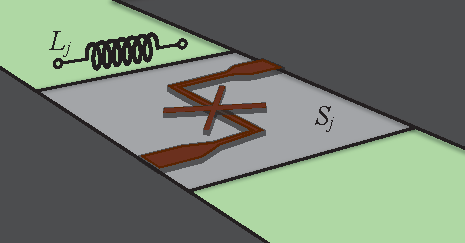
\includegraphics[scale=1.1]{methods/FE-junc} \caption[Finite-element model of linearized Josephson junction]{\textbf{Finite-element model of linearized Josephson junction.}\label{fig:Appdx:JJ-FE-model}
Not-to-scale schematic representation of the finite-element model
of the linearized Josephson junction (location marked by cross) connected
by wire leads (elevated brown trace) to two large metal pads (dark
rectangles). Since the geometry of the junction and leads is in deep-sub-wavelength
regime, it can typically be ignored, and the inductance presented
by the junction, $L_{j}$, graphically represented by black inductor
symbol with two open terminals, can be modeled by a single lumped-element
inductive sheet, $S_{j}$, in the FE simulation, depicted by light
grey rectangle. Green background represents the substrate.}
\end{figure}

After the design geometry and boundary conditions are established,
 additional fine-mesh operations on crucial features of interest,
such as the junction rectangles, are applied to speed up the solver
convergence, which can be diagnosed by examining the parameters $\omega_{m}$
and $p_{mj}$ as a function of adaptive pass number. At each pass,
the FE solver provides the modal frequencies, $\omega_{m},$ and the
electric, $\vec{E}_{\mathrm{max}}(\vec{r})$, and magnetic, $\vec{H}_{\mathrm{max}}(\vec{r})$,
phasors. The electric field at a point $\vec{r}$ in the volume of
the device, $V$, at time $t$ is 
\[
\vec{E}\left(\vec{r},t\right)=\mathrm{Re}\,\vec{E}_{\mathrm{max}}\left(x,y,z\right)e^{j\omega_{m}t}\,.
\]
The total magnetic and electric field energies of a mode can be computed
from the eigenfields \citep{Pozar}:
\begin{eqnarray}
\mathcal{E}_{\mathrm{elec}} & = & \frac{1}{4}\mathrm{Re}\int_{V}\mathrm{d}v\vec{E}_{\text{max}}^{*}\overleftrightarrow{\epsilon}\vec{E}_{\text{max}}\;,\label{eq:app:FE:  W_E  W_H  integrals}\\
\mathcal{E}_{\mathrm{mag}} & = & \frac{1}{4}\mathrm{Re}\int_{V}\mathrm{d}v\vec{H}_{\text{max}}^{*}\overleftrightarrow{\mu}\vec{H}_{\text{max}}\;,\label{eq:app:FE:  W_H  integral}
\end{eqnarray}
where the spatial integral is performed over total volume, $V$, of
the device, and $\overleftrightarrow{\epsilon}$ ($\overleftrightarrow{\mu}$)
is the electric-permittivity (magnetic-permeability) tensor. While
the magnetic and electric energies are typically equal on resonance
\citep{Pozar}, when lumped elements are included in the model, the
more general equality is between the capacitive, $\mathcal{E}_{\mathrm{cap}},$
and inductive, $\mathcal{E}_{\mathrm{ind}},$ energies, $\mathcal{E}_{\mathrm{cap}}=\mathcal{E}_{\mathrm{ind}}\,.$
For our design, the capacitive energy is stored entirely in the electric
fields, $\mathcal{E}_{\mathrm{cap}}=\mathcal{E}_{\mathrm{elec}}$,
but the inductive energy is stored both in the magnetic fields and
in the kinetic inductance of the Josephson junctions, $\mathcal{E}_{\mathrm{mag}}=\mathcal{E}_{\mathrm{ind}}+\mathcal{E}_{\mathrm{kin}}$,
where $\mathcal{E}_{\mathrm{kin}}$ is the total energy stored in
the kinetic inductors, $\mathcal{H}-\mathcal{H}_{\mathrm{EM}}$, see
Eq.~(\ref{eq:HLin}); it follows, 
\begin{equation}
\mathcal{E}_{\mathrm{cap}}=\mathcal{E}_{\mathrm{ind}}+\mathcal{E}_{\mathrm{kin}}\,,\label{eq:CapIndKinEnegry}
\end{equation}
which, for a single-junction device, implies that the EPR of the junction
in mode $m$ is 
\begin{equation}
p_{m}=\frac{\mathcal{E}_{\mathrm{elec}}-\mathcal{E}_{\mathrm{mag}}}{\mathcal{E}_{\mathrm{elec}}}\:.
\end{equation}
For a device with multiple junctions, such as the Darkmon, it follows
from Eq.~(\ref{eq:EPR-defn-verbal}), that the EPR of junction $j$
in mode $m$ is 
\begin{equation}
p_{mj}=\frac{1}{2}L_{j}I_{mj}{}^{2}/\mathcal{E}_{\mathrm{ind}}\;,\label{eq:appx:FE:pmj}
\end{equation}
where $I_{mj}$ is the junction peak current, which can be calculated
from the surface-current density, $\vec{J_{s}^{m}}$, of the junction
sheet $S_{j}$, 
\begin{equation}
\left|I_{mj}\right|=l_{j}^{-1}\int_{S_{j}}\mathrm{d}s\left|\vec{J_{s}^{m}}\right|\;,\label{eq:appx:FE:ImjAbs}
\end{equation}
where $l_{j}$ is the length of the sheet, see Fig.~\ref{fig:appx:FE JJsurf}.

\begin{figure}[ht]
\centering{}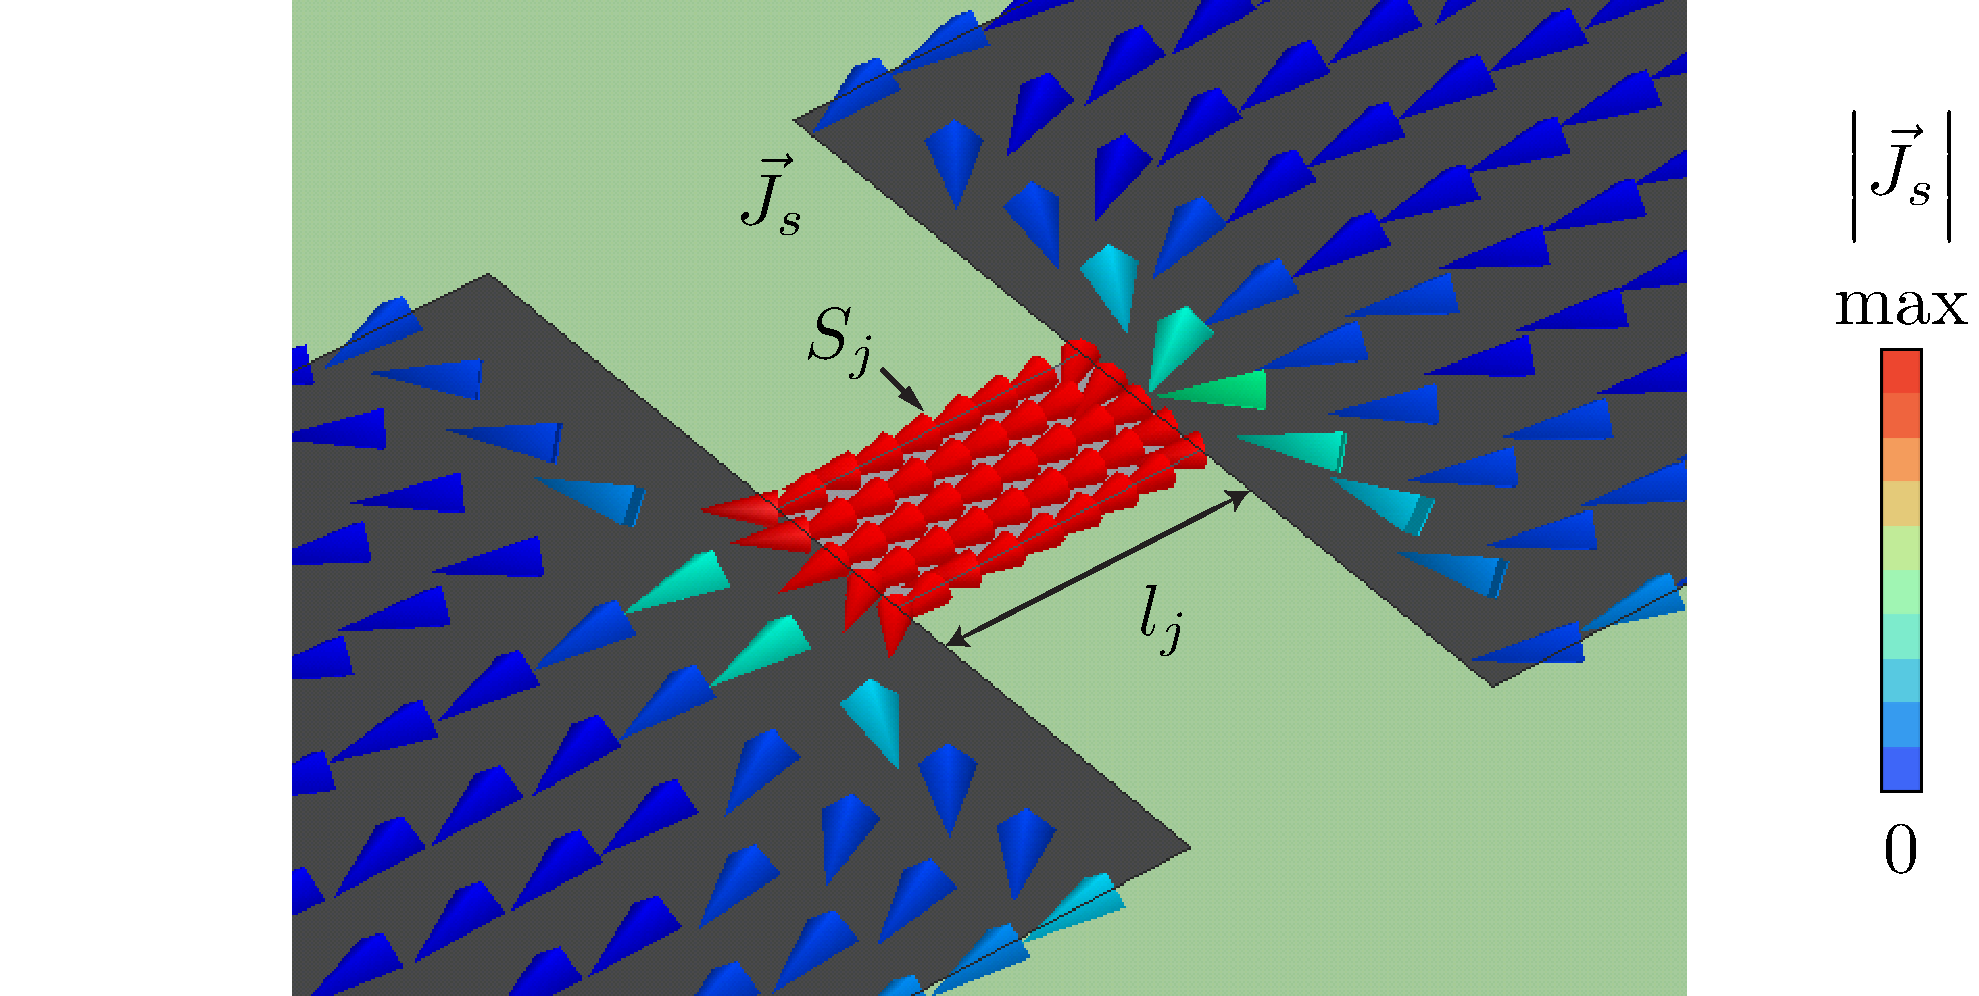
\includegraphics[width=4.3in]{methods/appx_FE_JJsurf}
\caption[Finite-element simulation of a transmon device]{\label{fig:appx:FE JJsurf}\textbf{Finite-element simulation of a
transmon device.} Plot of the surface-current density, $\vec{J}_{S}$,
of a transmon qubit mode, obtained with finite-element electromagnetic
eigenmode simulation; red (blue) indicates maximum (minimum) current
magnitude. Josephson junction (center rectangle) is modeled by a single
inductive sheet ($S_{j}$) with length $l_{j}$, spanning the distance
between the two transmon pads (dark rectangles). Green background
represents the transmon chip. }
\end{figure}

The calculation of the EPR sign bits, $S_{mj}\in\left\{ -1,1\right\} $,
requires the definition of a convention for the junction orientation,
which is accomplished by supplementing the FE model with a directed
line, $\mathrm{DL}_{j}$, along the length of the junction sheet $S_{j}$.
The actual orientation of the line is irrelevant, so long as it spans
the two terminals of the junction. The sign of the current along the
line can be used as the sign bit 
\begin{equation}
S_{mj}=\sign\int_{\mathrm{DL}_{j}}\mathrm{d}\vec{l}\cdot\vec{J_{s}^{m}}\;.\label{eq:app:Smj calc}
\end{equation}


\paragraph{Remarks.}

The convergence of the EPR extracted from local field quantities,
$I_{mj},$ can be enhanced by renormalizing the EPRs so as to enforce
the global condition given by Eq.~(\ref{eq:CapIndKinEnegry}), $\sum_{j\in J}p_{mj}=\mathcal{E}_{\mathrm{kin}}/\mathcal{E}_{\mathrm{ind}}$.
The eigenmode simulation approach affords several distinct advantages.
No prior knowledge of the mode frequencies is required to execute
the simulation. The solver can be queried to solve for the $N$-lowest
eigenmodes. If only information on modes above a particular frequency
is desired, this cutoff frequency can also be supplied to the solver.
From a single mesh and simulation, the FE solver returns \emph{complete}
information for all modes of interest — the parameters $\omega_{m}$,
$p_{mj},$ and $S_{mj}$ of the Hamiltonian and, as shown in Sec.~\ref{subsec:Dissipation-budget},
the dissipation budget. These features play nicely into the iterative
nature of the design optimization, and make the eigenmode design-optimization
process easy to automate, provided freely to the community in our
software package pyEPR.\footnote{http://github.com/zlatko-minev/pyEPR}
In the optimization of the Drakmon device, the finite-element software
of choice was \emph{Ansys high-frequency electromagnetic-field simulator}
\emph{(HFSS)}.

\subsection{Calculation of Hamiltonian parameters with the EPR\label{subsec:Calculation-of-Hamiltonian}}

The quantities $\omega_{m}$, $p_{mj},$ and $S_{mj}$ obtained from
the FE eigenmode solution together with Eqs.~(\ref{eq:multijj:ZPF defn}),
and~(\ref{eq:pmj_multi_zpf}) completely specify $\hat{H}_{\mathrm{nl}}$,
Eq.~(\ref{ex:Hnl-multi}). The multitude of non-linear interactions
contained in $\hat{H}_{\mathrm{nl}}$ mix the LJC modes. However,
operating the Darkmon in the dispersive regime \citep{Blais2004,Koch2007},
defined by $\omega_{k}-\omega_{m}\gg E_{j}c_{jp}\left<\hat{\phi}_{j}^{p}\right>$
for all $p\geq3$, we can restrict our attention to the leading order
correction of $\hat{H}_{\mathrm{nl}}$ to $\hat{H}_{\mathrm{lin}}$
to account for the device spectrum, see level diagram of Fig.~\ref{fig:Darkmon-energy-level-diagram}.
The leading-order correction is given by the $p=4$ terms that survive
the rotating-wave approximation (RWA) \citep{Carmichael2008-Book2,Gardiner2004},
representing energy-conserving interactions. To leading order, in
the RWA, after normal-ordering, $\hat{H}_{\mathrm{nl}}$ reduces to
the effective Hamiltonian 
\begin{equation}
\hat{\overline{H}}_{4}/\hbar=-\sum_{m\in M}\Delta_{m}\hat{a}_{m}^{\dagger}\hat{a}_{m}+\frac{\alpha_{m}}{2}\hat{a}_{m}^{\dagger2}\hat{a}_{m}^{2}+\frac{1}{2}\sum_{m\neq n}\chi_{mn}\hat{a}_{m}^{\dagger}\hat{a}_{m}\hat{a}_{n}^{\dagger}\hat{a}_{n}\,,\label{eq:H4 - RWA main}
\end{equation}
which when combined with $\hat{H}_{\mathrm{lin}}$, Eq.~(\ref{eq:Hlin-multi}),
yields Eq.~(\ref{eq:HDarkmon}). The Lamb shift, $\Delta_{m}=\frac{1}{2}\sum_{n\in M}\chi_{mn}\,,$
represents the dressing of the linear mode $m$ by the zero-point
vacuum energy of all $M$ modes. From Eq.~(\ref{eq:H4 - RWA main}),
it follows that the measured transition frequency between $\G$ and
$\B$ is $\omega_{\mathrm{BG}}=\omega_{\mathrm{B}}-\Delta_{\mathrm{B}},$
where $\omega_{\mathrm{B}}$ is the LJC Bright eigenmode frequency
and $\Delta_{\mathrm{B}}$ is the Bright mode Lamb shift; a similar
conclusion holds for the GD transition. The Kerr frequencies are found
from the EPR,
\begin{equation}
\chi_{mn}=-\sum_{j\in J}\frac{\hbar\omega_{m}\omega_{n}}{4E_{j}}p_{mj}p_{nj}\label{eq:chi_mj=00003D}
\end{equation}
and $\alpha_{m}=\chi_{mm}/2$. Remarkably, from Eq.~(\ref{eq:chi_mj=00003D})
it becomes evident that the EPRs are essentially the only free parameters
subject to optimization and design in engineering the non-linear couplings,
since the frequencies, $\omega_{m}$, and Josephson energies, $E_{j}$,
are constrained to a narrow range due to practical considerations.
Notably, Eq.~(\ref{eq:chi_mj=00003D}) embodies the structure of
a spatial-mode overlap in the EPRs. 


\subsection{Calculation of dissipation budget with the EPR \label{subsec:Dissipation-budget}}

In this subsection, we summarize the methodology employed in minimizing
dissipation in the Darkmon device. This is achieved by optimizing
the geometry of the design (in parallel with the Hamiltonian parameter
optimization) with the aim of minimizing the susceptibility of each
mode to the various unavoidable material and input–output losses.
For each design variation, we compute the bound on the modal quality
factors by constructing a \emph{dissipation budget}, which consists
of the loss expected due to each lossy element in the design. By manipulating
the geometry, the budget can be favorably altered, to a degree. The
calculation of the dissipation parameters is detailed in the following. 

Losses can be classified as either \emph{capacitive, }proportional
to the electric field intensity, $\left|\vec{E}\right|^{2}$, or \emph{inductive},
proportional to the magnetic field intensity, $\left|\vec{H}\right|^{2}$.
The total loss due to a material is proportional to its energy participation
in the mode, $p^{l}$, a geometric quantity related to the field distribution,
and its intrinsic quality, $Q$, a material property. The intrinsic
material quality, $Q$, can typically only be bounded, while $p^{l}$
can be calculated from the eigenfields. The total capacitive and inductive
losses, characterized by $Q_{\text{cap}}$ and $Q_{\text{ind}},$
respectively, sum together with the loss due to input-output coupling,
$Q_{\mathrm{rad}}$, and give the upper bound on the quality factor
of an EM mode, $Q_{\text{total}}$, \citep{Zmuidzinas2012,Geerlings2013,Reagor2016}
\begin{equation}
\frac{1}{Q_{\text{total}}}=\frac{1}{Q_{\text{cap}}}+\frac{1}{Q_{\text{ind}}}+\frac{1}{Q_{\text{rad}}}\,.
\end{equation}
In the following, we explicate the calculation of each quantity. We
note that the EPR treats dissipation and Hamiltonian parameters on
equal footing, and all quantities, Hamiltonian and dissipative, are
extracted from a single eigensolution. 

\paragraph{Capacitive losses.}

Capacitive losses, proportional to the intensity of the electric field,
$\left|\vec{E}\right|^{2}$, can originate from bulk or surface of
materials. Dielectrics, such as the substrate of the Darkmon device,
constitute the primary source of bulk loss \citep{Martinis2014,Dial2016,Kamal2016-anneal},
and, unfortunately, every surface in a device possesses a near-unavoidable,
lossy, surface dielectric layer, possibly due to chemical residues,
condensation, dust, etc. \citep{Martinis2014,Wang2015}. Regardless
of the microscopic origin of the dielectric losses, the loss properties
of the $l$-th dielectric are characterized by a catch-all quality
factor $Q_{\text{cap}}^{l}$ (or equivalently the inverse of the loss
tangent) and the EPR of the dielectric in the mode, $p_{\mathrm{cap}}^{l}$
— the fraction of capacitive energy stored in dielectric element $l$.
For a bulk dielectric, the dissipative EPR is given by 
\begin{equation}
p_{\text{cap,bulk}}^{l}=\frac{1}{\mathcal{E}_{\mathrm{elec}}}\frac{1}{4}\mathrm{Re}\int_{V_{l}}\mathrm{d}v\vec{E}_{\text{max}}^{*}\overleftrightarrow{\epsilon}\vec{E}_{\text{max}}\,,
\end{equation}
where the integral is carried over the volume of the $l$-th dielectric
element, namely $V_{l}$. The dissipative EPR of a surface dielectric,
$p_{\mathrm{cap,surf}}^{l}$, can be approximated by 
\begin{equation}
p_{\text{cap,surf}}^{l}=\frac{1}{\mathcal{E}_{\mathrm{elec}}}\frac{t_{l}\epsilon_{l}}{4}\mathrm{Re}\int_{\text{surf}_{l}}\mathrm{d}s\left|\vec{E}_{\text{max}}\right|^{2}\,,
\end{equation}
where the surface layer thickness is $t_{l}$, and its dielectric
permittivity is $\epsilon_{l}$. The total capacitive loss in the
mode is the EPR-weighted sum of the individual contributions \citep{Zmuidzinas2012,Geerlings2013},
\begin{equation}
\frac{1}{Q_{\text{cap}}}=\sum_{l}{\frac{p_{\text{cap}}^{l}}{Q_{\text{cap}}^{l}}}\,.\label{eq:cap-loss}
\end{equation}


\paragraph{Inductive losses.}

Electric currents flowing in metals or metal-metal seams can result
in inductive losses. The bound on the mode inductive-loss quality
factor $Q_{\text{ind}}$ is a weighted sum of the intrinsic material
quality $Q_{\text{ind}}^{l}$ of each lossy inductive element $l$,
analogous to Eq.~(\ref{eq:cap-loss}), 
\begin{equation}
\frac{1}{Q_{\text{ind}}}=\sum_{l}{\frac{p_{\text{ind}}^{l}}{Q_{\text{ind}}^{l}}}\;,
\end{equation}
where $p_{\text{ind}}^{l}$ is the inductive-loss EPR of element $l$.
For a metal surface, this can be calculated from the eigenfield solutions,
\begin{equation}
p_{\text{ind,surf}}^{l}=\frac{1}{\mathcal{E}_{\mathrm{mag}}}\frac{\lambda_{0}\mu_{l}}{4}\mathrm{Re}\int_{\text{surf}_{l}}\mathrm{d}s\left|\vec{H}_{\text{max},\parallel}\right|^{2}\;,\label{eq:appx:dissip:p ind surf}
\end{equation}
where $\lambda_{0}$ is the metal skin depth at $\omega_{m}$, and
$\mu_{l}$ is the magnetic permeability of the surface (typically,
$\mu_{l}=\mu_{0}$). In the case of superconductors $p_{\text{ind,surf}}^{l}$
is the kinetic inductance fraction \citep{Gao2008,Zmuidzinas2012},
commonly denoted $\alpha$. Normal metals typically have an inductive
quality factor $Q_{\text{ind,surf}}^{l}$ of approximately one \citep{Pozar}.
Bulk superconducting aluminum has been measured to have an inductive
quality factor $Q_{\text{ind,surf}}$ bounded to be better than a
few thousand \citep{Reagor2013}. Meanwhile, the bound on the quality
of thin-film Al has been measured to be better than $10^{5}$ \citep{Minev2013}. 

\subparagraph{Seam losses. }

A distinct loss mechanisms occurs at the seam of two metals \citep{Brecht2015}.
For instance, a common source of such loss is the seam used in superconducting
cavities. In the FE model, the seam can be modeled by a line, denoted
$\text{seam}_{l}$, between the two mating metallic surfaces. The
seam inductive participation is 
\begin{equation}
p_{\text{ind,seam}}^{l}=\frac{1}{\mathcal{E}_{\mathrm{mag}}}\frac{\lambda_{0}t_{l}\mu_{l}}{4}\mathrm{Re}\int_{\text{seam}_{l}}\mathrm{d}l\left|\vec{H}_{\text{max},\perp}\right|^{2}\;,\label{eq:Pseam}
\end{equation}
where the seam thickness is denoted $t_{l}$, its magnetic permeability
$\mu_{l}$, and its the penetration depth $\lambda_{0}$. It is convenient
to recast the seam loss contribution 
\begin{equation}
\frac{p_{\text{ind,seam}}^{l}}{Q_{\text{seam}}}=\frac{1}{g_{\text{seam}}}\frac{\int_{\text{seam}}\left|\vec{J}_{s}\times\vec{l}\right|^{2}dl}{\omega\mu_{0}\int_{\text{vol}}\left|H_{\text{max}}\right|^{2}dV}\;,
\end{equation}
in terms of a seam admittance $g_{\text{seam}}$, which is defined
in Ref.~\citet{Brecht2015}.


\section{Sample fabrication\label{sec:Fabrication-of-sample}}

Samples were fabricated on 430~$\text{\ensuremath{\mu}}$m thick,
double-side-polished, c-plane sapphire wafers, grown with the edge-defined
film-fed growth (EFG) technique, with the bridge-free junction fabrication
method, see Refs. \citet{Lecocq2011-bridge-free,Pop2012-Junction,Pop2011-Thesis,Reagor2016}.
We defined the sample pattern, both large and fine structures, with
a 100~kV electron-beam pattern generator (\emph{Raith EBPG 5000+})
in a single step on a PMAA/MAA resist bilayer. In the following,
we describe each step of the fabrication process in detail, and we
hope that by adding some additional information about each step and
motivation behind it, a reader who is new to the subject will benefit. 

\paragraph{Cleaning the wafer. }

First, the sapphire wafer is solvent cleaned under a chemical hood
in a two-step $N$-Methyl-2-pyrrolidone (NMP) process. The solvent
removes dust, organic residues, and oils on the wafer surface. For
our samples, we heated the wafer to $90\ensuremath{~\ensuremath{^{\circ}}\text{C}}$
for 10 minutes in an NMP bath, then sonicated it in the bath for another
10~minutes. After removing the wafer from the bath, if it is left
out to dry on its own, the NMP would evaporate quickly and leave undesirable
residue behind. Instead, we rinsed the wafer in an acetone bath, followed
by a methanol one, before finally blow drying it with filtered nitrogen
gas. Methanol has low evaporation pressure and under the blow drying
tends to take away the residues, rather than simply evaporating and
leaving residues behind. An acid should not be used to clean the sapphire
wafer, since the wafer is costly and already polished.


\paragraph{Spinning the positive resist bi-layer. }

The copolymer resist (\emph{Microchem} \emph{EL-13}) is spun onto
the cleaned wafer at 2,000~revolutions per minute (r.p.m.) for 100
seconds,  then, it is baked for 5~minutes at $200~\ensuremath{^{\circ}}\text{C}$.
The PMMA resist (\emph{Microchem A-4}) is spun on top of the first
at 2000~r.p.m. for 100~seconds. The wafer is baked at $200~\ensuremath{^{\circ}}\text{C}$
for 15~minutes, yielding a thickness of about 200~nm. It is worth
noting why PMMA is the resist of choice: it offers high, nm-sized
resolution, simplicity and ease of handling, no sensitivity to white
light, nor shelf or film life issues, and is easily dissolved, qualities
that make it the ideal resist for this type of nanofabrication.

Before proceeding to patterning, fabrication on sapphire requires
an extra step: the anti-charging layer. Whereas most silicon substrates
are conducive enough to prevent electron beam deflection during the
e-beam writing, sapphire substrates are not. The buildup of charge
is mitigated by depositing  a thin (10~nm) anti-charging layer of
gold on the wafer. In terms of metals, gold is an excellent choice,
as it is inert, does not have an oxide, and has notably high electrical
conductivity. Alternatively, we have also used aluminum for the anti-charging
layer (13~nm thick). 

\paragraph{Writing and developing the pattern. }

Both large and fine structures, including the Josephson tunnel junction
are patterned in a single step with the 100~kV EBPG, following which,
the gold layer is removed by submerging the wafer in a potassium-iodide/iodine
etch solution for 10~seconds. Next, the wafer is rinsed in water
and the resist is developed in a 3:1~IPA:water mixture at $6~\ensuremath{^{\circ}}\text{C}$
for 2~minutes. After development, the pattern is inspected under
an optical microscope. 


\paragraph{Plasma cleaning, deposition, and oxidation. }

The wafer is loaded in the electron-beam evaporation system, a multi-chamber\emph{
Plassys UMS300 UHV}. To prepare the surfaces for deposition and reduce
the amount of aging of the Josephson junction, the exposed sample
surfaces are subjected to a 1~minute of oxygen-argon plasma cleaning,
under a pressure of $3\times10^{-3}$~mbar. In this procedure, the
etch removed 30~nm from the upper resist layer; however, ideally,
one would use a shorter duration and larger pressure \citep{Pop2012-Junction},
which was not available. Next, the sample is transferred from the
load-lock to the deposition chamber, where an automated titanium sweep
is performed to absorb residual gases in the deposition chamber. 
At an angle of $19$~degrees, 20~nm of Aluminum is deposited onto
the sample, following which, the sample is transferred to the oxidation
chamber, where it is exposed to a 3:17 oxygen:argon mixture for 10~minutes
at 100~Torr. This forms an approximately 1~nm thick aluminum oxide
layer, the insulating barrier of the $\text{Al/Al\ensuremath{\mathrm{O}_{\mathrm{x}}}/Al}$
Josephson tunnel junctions. The sample is returned to the deposition
chamber, where the second and final layer of aluminum (30~nm) is
deposited at an angle of $-19$~degrees. Next, rather than directly
removing the sample from the evaporation system and allowing the exposed
aluminum surfaces to uncontrollably oxidize in air, the surfaces are
passivated with a final oxidation step at 50~Torr for 10~minutes.
The aluminum forms a self-limiting oxide capping layer.

\paragraph{Liftoff.}

The sample is placed in a heated bath of NMP solvent at $70~\ensuremath{^{\circ}}\text{C}$
for two hours. It is then sonicated for 1~minute, while still in
the NMP, following which, the NMP is cleaned with acetone, methanol,
IPA, and, finally, a dry nitrogen blow gun. The solvent ``lifts off''
the unwanted metal from the wafer by dissolving the resist underneath
it, thus leaving the bath full of aluminum flakes. Note that NMP
can't be heated much above $100~\ensuremath{^{\circ}}\text{C}$, since
that will likely damage the $\text{Al/Al\ensuremath{\mathrm{O}_{\mathrm{x}}}/Al}$
junctions.  

\paragraph{Dicing.}

A protective coating of optical resist (\emph{SC1827}) is spun at
1,500~r.p.m. for 120~seconds and baked at $90~\ensuremath{^{\circ}}\text{C}$
for 5~minutes. The sample is loaded in the dicer (\emph{ADT ProVecturs
7100}), which then is calibrated, aligned, and which then performs
the dicing. The diced chips are cleaned with acetone, methanol, and
dry nitrogen, and are stored until they ready to be mounted in the
sample holder. 

\paragraph*{Sample selection.}

The diced chips are cleaned (NMP, Acetone, methanol, nitrogen air)
and visually examined under an optical microscope where the normal-state
resistance, $R_{N}$, of their Josephson junctions is measured. This
is performed under an optical microscope (\emph{Copra Optical Inc.
SMZ800}) with probe needles (\emph{Quater-Research H-20242}) lowered
to contact the transmon pads on either side of the junction, taking
care to properly ground all object in contact with the sample and
to minimize unavoidable scratching of the pad during the probing.
The measurement of $R_{N}$ provides a good estimate of the junction
Josephson energy, $E_{J}$, by an extrapolation from room temperature
to the operating sample temperature, at approximately $15$~mK, using
the Ambegaokar-Baratoff relation \citep{Ambegaokar1963},
\begin{equation}
E_{J}=\frac{1}{2}\frac{h\Delta}{\left(2e\right)^{2}}R_{N}^{-1},
\end{equation}
where $\Delta$ is the superconducting gap of aluminum. The chip
closest matching the Josephson energies, $E_{J}$, of the EPR-designed
vertical and horizontal junctions is selected for mounting in the
sample holder. 

\section{Sample holder \label{sec:Sample-holder-materials}}

In this section, we describe the methodology used in the design of
the sample holder and readout cavity, while paying special attention
to the motivation underlying the design choices. The boundary conditions
of the readout cavity, depicted in Fig.~\ref{fig:setup}, are formed
from the superconducting inner walls of the chip sample holder, composed
of two main halves, see Fig.~\ref{fig:Sample-holder-and-pins}c,
and based on the ideas presented in Ref.~\citet{Paik2011}. Before
a discussion on the design geometry, we focus on the selection of
its materials.

\subsection{Material losses and selection \label{subsec:sample-holder-material-selection}}

\paragraph{Readout cavity considerations.}

The inner walls of the sample holder establish the boundary conditions
of the readout cavity mode, and hence have a large inductive, $p_{\text{ind,surf}}^{l}$,
and dielectric, $p_{\text{cap,surf}}^{l},$ surface-loss participation
ratio, see Sec.~\ref{subsec:Dissipation-budget}. It follows that
the material quality of the cavity inner walls is important in determining
the readout quality factor, $Q_{\mathrm{R}}$. However, since this
mode is purposefully made low-Q, by coupling it strongly to the input-output
(\emph{I-O}) couplers, the importance of the sample-wall material
is greatly reduced, and could in principle be rather lossy. For instance,
in some designs, copper, which has an inductive quality factor of
unity,  $Q=1$, has been used, thus limiting $Q_{\mathrm{R}}$ to
several thousand. Under these conditions, a fraction of the readout
cavity signal is lost to the walls of the cavity, rather than to the
\emph{I-O} couplers. Nonetheless, the \emph{I-O} coupling is engineered
to be larger still, so that most of the signal in the readout cavity
makes it to the amplifier chain, and a high quantum measurement efficiency,
$\eta$, can still be obtained. 

\paragraph{Qubit mode considerations. }

However, the Bright and Dark qubit modes, while predominantly spatially
localized to the sapphire substrate region, have a small fraction
of their fields extending to the inner walls of the readout cavity.
Although the lossy energy participation ratios, $p_{\text{ind,surf}}^{l}$
and $p_{\text{cap,surf}}^{l}$, are exponentially small ($\lesssim10^{-5}$),
so that the cavity walls participate on the part-per-million level,
a normal-metal wall ($Q_{\mathrm{ind}}^{l}\approx1$) could limit
the qubit quality factors significantly, making lifetimes on the order
of $T_{\mathrm{1}}^{\mathrm{D}}\approx100\ \mathrm{\mu s}$ out of
reach. For this reason, we employ a low-loss superconducting material
for the sample holder, and clean its surfaces with care, see discussion
on Pg.~\pageref{par: Surface-preparation}. Specifically, we machined
the readout cavity from 6061 aluminum alloy, which is typically found
in the construction of aircraft structures. Notably, it is a good
superconductor, and due to its hardened structure offers a machining
advantage over regular aluminum, which is too soft. 

We remark that in other experiments, involving high-Q storage mode
cavities, the cavities are often machined from high-purity 4N (99.99\%
pure) aluminum (or sometimes, 5N), which is very soft, and thus difficult
to machine. Further, the machining forms deep cracks ($\approx100\ \mathrm{\mu m}$),
where machining oils and dirt seep in, and hence, the surfaces require
a more involved chemical etch process to remove about 150$\ \mathrm{\mu}$m
of the surface; see the dissertation of M. Reagor \citep{Reagor2016}.

\begin{figure}
\begin{centering}
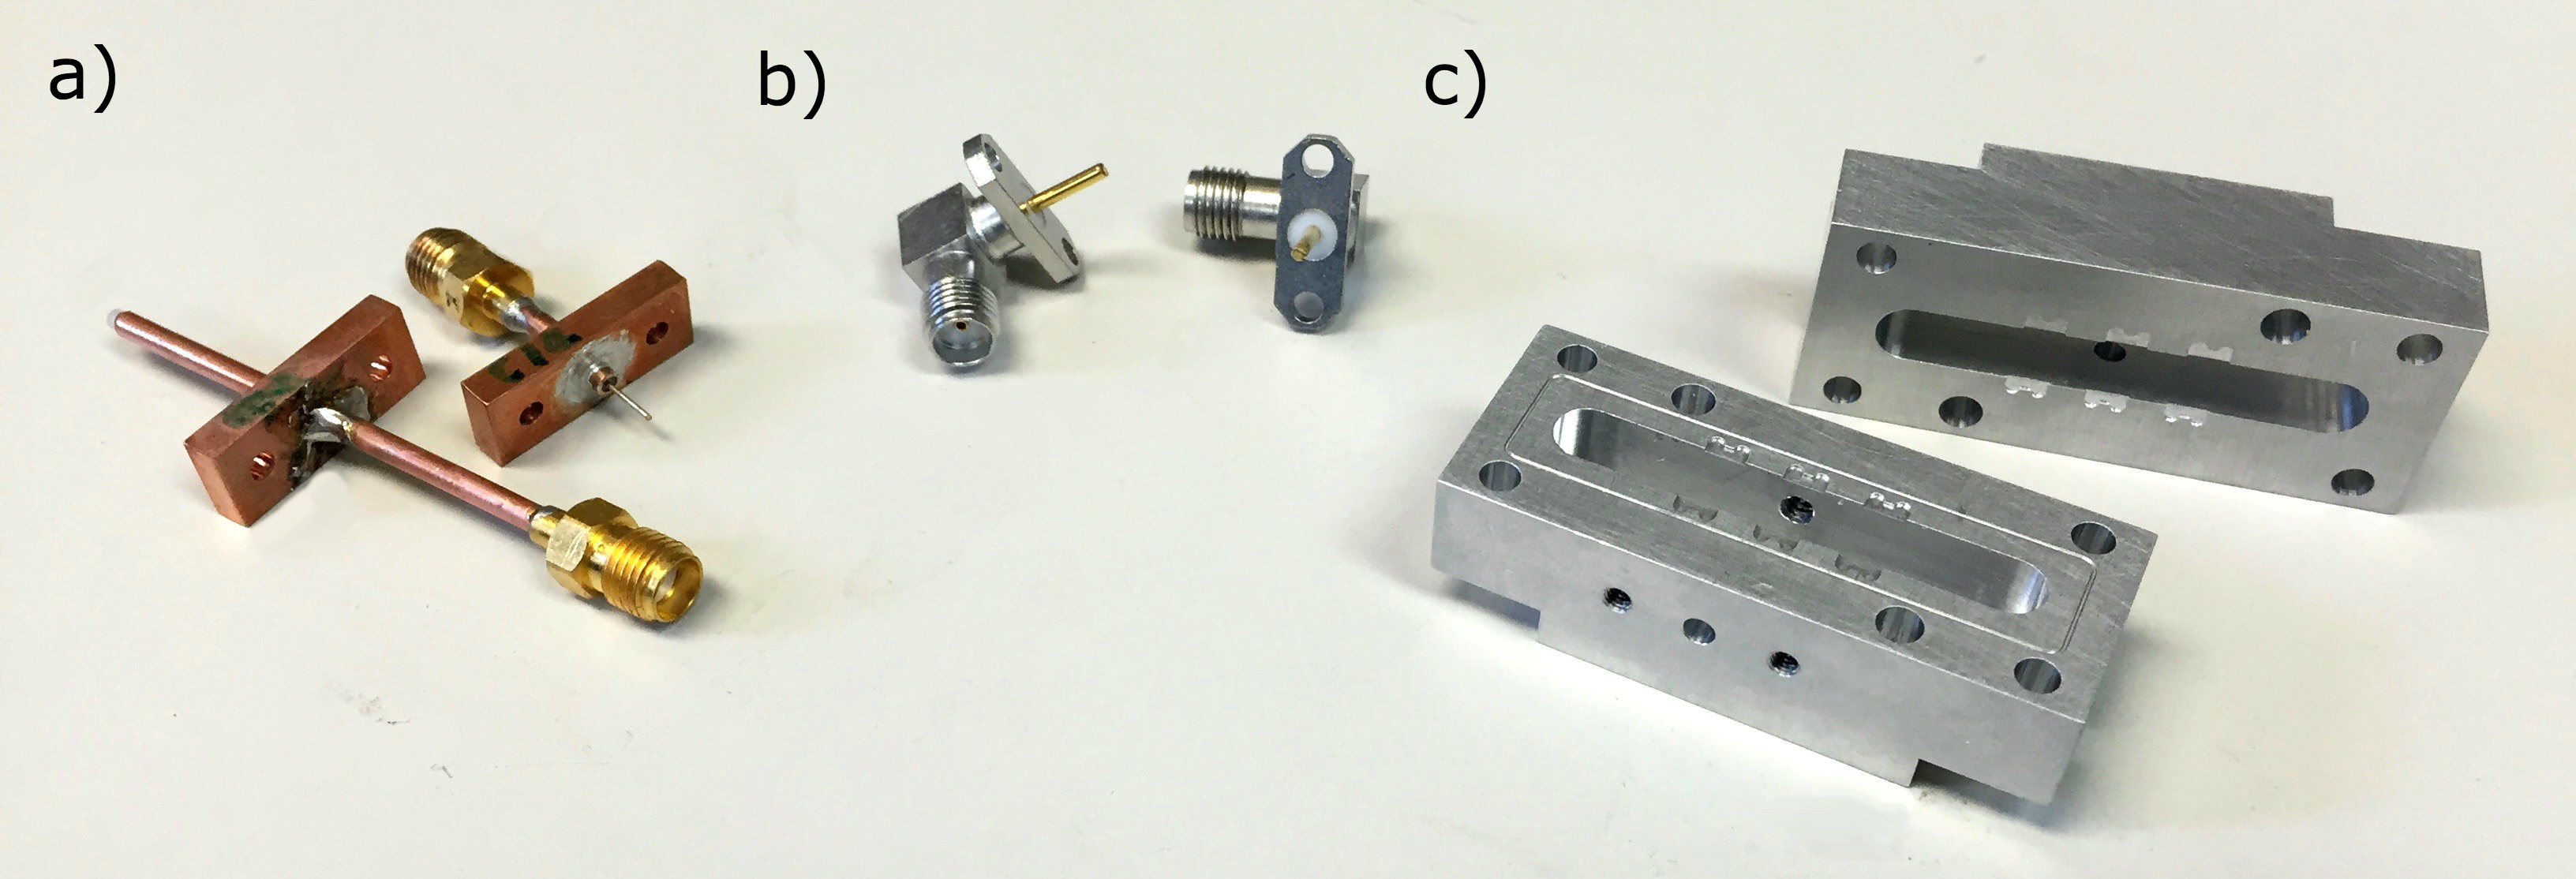
\includegraphics[width=1\columnwidth]{methods/sample_holder_and_pins_non_mag}
\par\end{centering}
\caption[Non-magnetic couplers and sampler holder ]{\label{fig:Sample-holder-and-pins}\textbf{Non-magnetic couplers
and sampler holder.} \textbf{a/b, }Photograph of two generations of
custom-made, non-magnetic, \emph{SubMiniature version A} (SMA), input-output
(\emph{I-O}) pin couplers. \textbf{c,} Photograph of disassembled
sample holder, inside walls forms boundary condition for the readout
cavity mode. Three machined grooves on the mating surfaces of the
two halves provide placement slots for samples. Mating surface of
lower-half has groove encircling the inside cavity, employed with
an indium wire to seal the two halves. Large through holes visible
on the mating surfaces provide means to fasten sample holder and attach
it to a cold finger in the dilution refrigerator. Small hole visible
on the interior back wall of the lower half allows for screw-tuning
of the readout cavity frequency.}
\end{figure}


\paragraph*{Non-magnetic input-output couplers.}

It has been recognized that commercial flange-based\emph{ I-O} couplers
contain magnetic ferrite impurities with fields at the ten milligauss
level, which although small, due to the close spatial proximity of
the coupler to the thin-film superconducting pads of the transmon,
as well as the Josephson junction, could introduce vortices in the
films, and it is suspected, generally degrade the superconductor performance.
To achieve better control of the electromagnetic environment and to
reduce potential losses due to magnetic impurities, we employed custom-made
pins from non-magnetic materials, such as copper and brass. 

Panels (a) and (b) of Fig.~\ref{fig:Sample-holder-and-pins} show
two generations of non-magnetic, \emph{SubMiniature version A} (SMA)
pin-couplers. The first generation, see panel (a), was made in-house
from a standard, SMA copper cable with two female connectors. After
testing the quality of the cable, by checking its insertion loss with
a vector network analyzer (VNA), the cable was cut in two, partially
stripped (external shielding and teflon) to expose the center conductor,
which serves as the pin inside the readout cavity, and soldered (non-magnetic
solder) to a custom copper flange. The flange can then be mounted
to the outside surface of the readout cavity, see panel (c), by non-magnetic,
brass or aluminum, screws. Panel (b) shows a second generation of
non-magnetic couplers, made from beryllium-copper, and custom-ordered,
courtesy of Christopher Axline. In general, components used with the
sample holder, placed inside the enclosing magnetic shielding, were
tested for magnetic compatibility with a magnetometer inside a magnetically
shielded box at room-temperature. 

\paragraph*{Sample-holder seam.}

To enclose the Darkmon chip in the sample holder, the sample holder
is designed as two separate halves, see Fig.~\ref{fig:Sample-holder-and-pins}c.
As discussed in Sec.~\ref{subsec:Dissipation-budget}, the placement
of the seam in the design is important, as it determines the seam-loss
participation ratio, $p_{\text{ind,seam}}^{l}$. The seam in placed
at the minimum of the current field profile of the readout cavity
mode. No perfect symmetry exists in the design; it is broken by the\emph{
I-O} couplers and the sample chip, so even at this location, the participation
is not strictly zero for either the readout cavity or qubit modes.
For this reason, it is important that the seam quality is as high
as possible. In the following, we remark on seam properties at the
microscopic level, and the use of an indium seal for improved electrical
contact.

\emph{Seam quality at the microscopic level.\label{disc:Seam-quality}
}Even under high pressure, applied by the fastening action of the
sample holder screws, see Fig.~\ref{fig:Sample-holder-and-pins}c,
the mating faces of the two halves of the sample holder do not join
well at the atomic level. Three interface regions can be identified:
i) \emph{metal-to-metal} \emph{regions}, the rarest, where aluminum
atoms from both halves are in physical contact, allowing superconducting
current to flow undisturbed, ii)\emph{ semi-conducting regions}, more
common, where contaminants, typically dielectric, result in resistive
conductance, and iii) \emph{non-conducting regions, }typically, the
most common, where electrical flow is altogether prohibited, for either
the region is a vacuum gap or is dominated by a thick non-conductive
film of oxides, sulphides, etc. The physical contact area is typically
less than a tenth of the area of the mating surfaces.

\emph{Higher-quality seam. }To create a seam with higher electrical
conductivity, one can first increase the force applied to form the
bond to fracture the native oxide layer of the mating surfaces and
to yield a greater physical contact area, region (i). However, this
method is rather limited in applicability with our design, because
the constraint of non-magnetic screws excludes nearly all hard-material
screws, including stainless steel ones, due to magnetic impurities.
The soft screws we use, aluminum and brass, lack the impurities needed
to make them withstand larger forces, and tend to break and strip
easily. Mostly, we relied on a soft-metal seal, a thin wire gasket
placed in a small groove in one of the mating faces. A number of materials
metals are conventionally used as soft-metal seals, such as copper,
aluminum, indium, etc. The seal of choice in the cQED community is
indium, typically used in cryogenic hermetic seals and low-temperature
solder with melting point of 47~°C, since it remains soft and malleable
even at cryogenic temperatures and is a superconductor. The indium
gasket has been observed to increase the internal quality factor of
a superconducting cavity by several orders of magnitude and its estimated
seam conductance is $g_{\mathrm{seam}}\gtrsim10^{6}/\mathrm{\Omega m}$
\citep{Brecht2017-Thesis}. In our experiment, we used an un-greased
99.99\% indium wire of 0.020~in. diameter to form the seam gasket.

\subsection{Assembly}

After the surfaces of the machined sample holder are cleaned, see
discussion on Pg.~\pageref{par: Surface-preparation}, the Darkmon
chip selected from the diced wafer, Sec.~\ref{sec:Fabrication-of-sample},
is cleaned (NMP, Acetone, methanol, nitrogen air) and, under an optical
microscope, is immediately placed in the central groove of the sample
holder, see Fig.~\ref{fig:Sample-design-assembly}a. The groove is
designed to be larger (at minimum 5\%) than the dimensions of the
chip to account for the differential thermal contraction between aluminum
and sapphire (mostly, the aluminum contracts) and machining tolerances.
The precision of the dicing saw (\emph{ADT ProVecturs 7100}) is high,
several microns when recently calibrated, and the chip will not exceed
the diced margin by more than a few microns, but it can fall quite
short of that, because, unlike silicon, when sapphire is diced, it
shatters around the edges, much like glass, and forms a jagged edge.
For this reason, when placed in the groove, the chip can rattle about,
and requires anchoring, accomplished by placing four small bits of
indium on its four corners and pressing them down to fill the corner
circular pockets machined in the groove, see Fig.~\ref{fig:Sample-holder-and-pins}c.
To minimize contamination during the mounting, the chip is placed
face down in the groove, although, we note that even dust on the back
side of the chip can contribute to loss in the qubit modes, though,
its participation ratio will be far smaller than if it were on the
front face. 

When the sample is well anchored, the indium gasket is laid down in
the gasket groove, as visible in Fig.~\ref{fig:Sample-design-assembly}a,
and the top half of the sample holder is mounted on top, fastened
tightly with even-pressure to allow the indium to distribute evenly.
For the screws, we used aircraft-alloy 7075 (\emph{McMaster}/\emph{Fastener
Express}), with less than 1\% iron impurities. These screws, as discussed
earlier, are rather soft, and to achieve a higher compression between
the two halves at cryogenic temperatures, we used the screws with
\label{par:molybdenum}molybdenum washers, which provide differential
contraction — the linear thermal contraction for molybdenum (aluminum)
between room temperature and 4~K is 0.095\% (0.415\%). Molybdenum
is compatible with the non-magnetic requirement. After 10 minutes,
the indium seal relaxes, and the screws can be further tightened,
with even pressure.


\section{Cryogenic setup\label{sec:Cryogenic-setup} }

The embedding environment of the sample is nearly as important as
the properties of the sample itself in achieving long-coherences and
desired performance. For this reason, in this section, we focus on
a few notable aspects of the cryogenic setup, and pay particular attention
to motivations. For the most part, our cryogenic setup is rather standard
in the field of cQED. For a more general discussion of low-temperature
cryogenics, see Refs.~\citet{ventura2010book} and \citet{pobell2013book}.

\subsection{Material selection\label{subsec:Material-selection}}

As already emphasized, the material selection of components used in
the setup is of prime importance. For this reason, we feel it worthwhile
to note a few overriding principles, corroborated by experience, employed
when selecting materials for the cryogenic setup of a cQED experiment,
which have to be compatible with operation at milikelvin temperatures
and high vacuum ($<10^{-1}$ \,Pa).

\paragraph{Tested and well-understood cryogenic materials. }

In the cryogenic setup of our experiment, we employed only materials
that have been exhaustively studied, characterized, and established
in regular laboratory use. There are only a handful suitable for cQED
experiments, which, in the solid-state, can classified as: i) ambient-pressure
superconductors: aluminum, niobium, indium, titanium, tin, molybdenum,
and niobium-titanium (NbTi), ii) normal metals: copper, brass, gold,
beryllium, stainless steel, and iii) dielectrics: silicon, sapphire,
quartz, nylon, Teflon, Stycast, poly(methyl methacrylate) (PMMA).
The listed materials are the most common ones; for material properties,
see Refs.~\citet{ventura2010book} and \citet{pobell2013book}. 

\paragraph*{Simplicity and homogeneity.}

The simplest and smallest number of materials were employed in the
cryogenic setup. The Darkmon sample (including \emph{I-O} pins, seam
gaskets, screws, \emph{et cetera})  consisted of essentially three
types of atoms — aluminum, oxygen, and indium. Beyond the materials
employed in the sample holder, the properties of commercial components
were found to vary among manufacturers, for instance, the residual
magnetic impurity levels measured in screws and SMA connectors, barrels,
adapters, \emph{et cetera} varied across manufacturers. For this reason,
prior to use in the setup, all components were screened with a magnetometer,
especially when employed inside magnetically shielded compartments.

\paragraph{Aluminum. }

Chief among the materials employed was aluminum (Al), and hence, we
pay special attention to its properties. From a structural standpoint,
Al is ``light-weight,'' having one-third the density and stiffness
of steel and copper. However, unlike steel, it is free of magnetic
impurities and has 59\% of the thermal and electrical conductivity
of copper at room temperature. Importantly, when aluminum oxidizes,
it forms a protective coating of amorphous aluminum oxide ($\mathrm{AlO_{x}}$)
that is thermodynamically favored to self limit growth to a thickness
of merely one nanometer. The $\mathrm{AlO_{x}}$ layer is special
in that it has one of the highest hardness coefficients of all oxides,
even greater than glass, making it an excellent (unavoidable) encapsulation
layer, rendering Al highly resistant to corrosion, but also making
the formation of a very-conductive Al-Al seam difficult, as discussed
on Pg.~\pageref{disc:Seam-quality}, and resulting in a surface dielectric
layer with a loss tangent, see Sec.~\ref{subsec:Dissipation-budget}.


\subsection{Thermalization}

The design and implementation of a high-thermal-conductivity link
between the Darkmon sample and the main source of cooling power in
the dilution refrigerator, the mixing chamber pot, is crucial to take
undesired heat away from the sample. At low temperatures, the task
is complicated since the rate limiting factor in the heat transfer
becomes the \emph{contact} \emph{thermal resistance, $R_{\mathrm{C}},$}
found at the interface of two mating surfaces, intricately dependent
upon on the interface properties and difficult to control. The temperature
discontinuity, $\Delta T$, across two mating surfaces is 
\begin{equation}
\Delta T=\frac{R_{\mathrm{C}}}{A}\dot{Q}\,,
\end{equation}
where $A$ is the surface area and $\dot{Q}$ is the power flowing
through the surface. It is seen that to minimize $\Delta T$ once
can increase the contact area, $A$, or decrease the geometry-independent
resistance, $R_{\mathrm{C}}.$ In the following, we describe the thermal
link setup of the sample and briefly outline the strategies employed
to minimize $R_{C}$ across the various interfaces.

\textbf{Gold plating and welding. }The sample was mounted on a cold-finger
attached to the mezzanine mixing-chamber plate. The plate is \emph{gold
plated }($\approx5\mu m$ by electroplating) to achieve higher thermal
conductivity. As a soft metal, gold allows for a larger 'real' surface-area
contact, and due to its chemical inertness, also provides protection
from oxidation of the surface, which keeps $R_{\mathrm{C}}$ low across
multiple uses and over time. The cold finger is not gold-plated, due
to the cost and long-lead time of the process. It is machined from
two oxygen-free high-thermal-conductivity (OFHC) copper blocks, which
are \emph{welded together }to minimize the number of contact joints,
essentially eliminating $R_{\mathrm{C}}$ altogether. Of course, the
bulk thermal resistance of the OFHC copper block remains, but it is
rather small and the cross-sectional area of the cold-finger block
is rather large, providing a good thermal link.

\textbf{Pressure and differential contraction. }The sample is fixed
to the cold finger with aluminum screws. The cold finger is mounted
on the mezzanine mixing-chamber plate with stainless steel screws,
which allow greater pressure. To maximize the pressure across all
joints, \emph{molybdenum washers }were used everywhere to provide
further differential-contraction pressure, see discussion on Pg.~\pageref{par:molybdenum}. 

\textbf{Thermal straps. }The cold finger thermalization link contains
several unavoidable joins, an issue that can be circumvented to a
degree with the use of a flexible heat strap (also known as \emph{thermal
braid}). Directly mounted on the sample was a small copper block welded
to a thick OFHC copper heat strap (models \emph{P6-501} and \emph{P7-501}
from \emph{TAI}) that extended to the mixing chamber plate without
interruption. The strap has the advantage of being durable, flexible,
and reusable.

\textbf{\label{par: Surface-preparation}Surface preparation. }The
physical and chemical condition of the surfaces forming the contact
determine $R_{\mathrm{C}}$. When a component is machined, the stresses
applied to the surface create dislocations and riddle the surface
with extremely narrow (order of a few nanometers) but deep (hundreds
of nanometers) cracks, into which machining oils seep. The cracks
and oil residues degrade the surface quality, visually, electrically,
and thermally. For this reason, all surfaces involved in forming a
thermal link were prepared in the following way. First, they were
cleaned abrasively with scotch bright, buffing, and  fine sandpaper,
removing the top surface layer and resulting in a shiny mirror finish.
Second, the mating component was cleaned chemically. Typically, by
sonication in an anionic detergent solution (\emph{Alconox 1\%}),
followed by acetone, then IPA, and finally blow dried with dry nitrogen
air. For more aggressive cleaning, we used a powerful oxidizing agent,
nitric acid ($\mathrm{HNO_{3}}$), to etch the surface. The acid and
oxidized impurities were then washed away with deionized water, followed
by an acetone and isopropanol (IPA) bath, and finally a nitrogen blow
dry. The components were then mounted immediately, before a substantial
oxide layer could form. For previously treated components that required
remounting, the mating surface was cleaned with blue solder flux,
which has a high concentration of nitric acid, immediately prior to
mounting.


\subsection{Light and magnetic shielding}

The quality factor of superconducting microwave aluminum resonators
(and qubits) is known to strongly depend on the quality of the infrared
and magnetic shielding of the embedding environment \citep{Barends2011-qp,Wang2014,Kreikebaum2016}.
Stray infrared light that is absorbed by a superconductor creates
quasiparticles, which reduces the overall quality factor of the superconducting
surface. This effect is especially pronounced in aluminum, whose superconducting
gap is rather low, $\approx88$~GHz \citep{Barends2011-qp,deVisser2011-qp}.
The effect of stray light can be largely mitigated with multistage
infrared shielding. Magnetic fields at the surface of the superconductor
can suppress the superconducting gap and introduce vortices, which
generally reduce the inductive surface quality, although, under certain
conditions, the vortices can act as quasiparticle traps, and can result
in overall higher quality \citep{Wang2014,Vool2014-qp}. 

\paragraph{Light shielding.}

Black-body radiation from warmer stages in the dilution refrigerator
was blocked by reflective thermal shields enclosing the mixing chamber
space and special care with taken to prevent line-of-sight leaks through
screw holes, \emph{et cetera}. However, \emph{low frequency} photons
are more difficult to shield against, and several further strategies
were employed to  make a light-tight sample space for the Darkmon
device. In addition to the indium seal between the two metal halves
of the sample holder, the sample holder was wrapped in three layers
of aluminized mylar foil, secured with copper tape. In some cooldowns,
the inside of the magnetic shield housing the sample (see below) was
lined with infrared absorbing epoxy \citep{Barends2011-qp,Rigetti2012}.
Coaxial thermalization and infrared filters (teflon replaced by\emph{
Eccosorb CR-110} as the dielectric) were used on the input and output
lines of the sample. 

\paragraph{Magnetic shielding. }

A high-magnetic-permeability, $\mu$-metal (\emph{Amumetal A4K}) can
enclosed an aluminum superconducting cylinder which housed the sample.
In this configuration, the $\mu$-metal shield allows the superconducting
shield to cool through its critical temperature in a lower magnetic
field, lowering the possibility of vortex trapping. Both shields were
thermally anchored to the mixing-chamber base plate by thermal straps,
while the $\mu$-metal shield was also anchored to the cold-finger
by direct contact. Components employed within the can were tested
for magnetic impurities with a magnetometer. Special care was taken
to avoid markings and paint that could be magnetic; paint on components,
such as directional couplers, was stripped with a solvent bath (typically,
Acetone). 


\section{Microwave setup\label{sec:Microwave-setup} }

\paragraph{Room temperature.}

The control tones depicted in Fig.~\ref{fig:setup} were each generated
from individual microwave generators ($\Omega_{\mathrm{D}}$ and $\Omega_{\mathrm{B0}}$:
\textit{Agilent N5183A}; readout cavity tone R and $\Omega_{\mathrm{B1}}$:
\textit{Vaunix LabBrick LMS-103-13} and LMS-802-13, respectively).
To achieve IQ control, the generated tones were mixed (\textit{Marki
Microwave Mixers IQ-0618LXP} for the cavity and \textit{IQ-0307LXP}
for $\Omega_{\mathrm{B0}},\Omega_{\mathrm{B1}}$, and $\Omega_{\mathrm{D}}$)
with intermediate-frequency (IF) signals synthesized by the 16 bit
digital-to-analog converters (DACs) of the integrated FPGA controller
system (\textit{Innovative Integration VPXI-ePC}). Prior to mixing,
each analog output was filtered by a $50\,\Omega$ low pass filter
(\textit{Mini-Circuits BLP-300+}) and attenuated by a minimum of 10\,dB.
The radio-frequency (RF) output was amplified at room temperature
(\textit{MiniCircuits ZVA-183-S+}) and filtered by \textit{Mini-Circuits}
coaxial bandpass filters. The output signal was further pulse modulated
by the FPGA with high-isolation SPST switches (\textit{Analog Device
HMC-C019}), which provided additional 80\,dB isolation when the control
drives were turned off. The signals were subsequently routed to the
input lines of the refrigerator. 

At room temperature, following the cryogenic high-electron mobility
amplifier (HEMT; \textit{Low Noise Factory LNF-LNC7\_10A}), the signal
were amplified by 28\,dB (\textit{Miteq AFS3-00101200-35-ULN}) before
being mixed down (\textit{Marki image reject double-balanced mixer
IRW-0618}) to an intermediate frequency (IF) of 50\,MHz, where they
were band-pass filtered (\textit{Mini-Circuits SIF-50+}) and further
amplified by a cascaded preamplifier (\textit{Stanford Research Systems
SR445A}), before finally digitization by the FPGA analog-to-digital
converters (ADC).


\paragraph{Cryogenic.}

The experiments were carried out in a cryogen-free dilution refrigerator
(\textit{Oxford Triton 200}). Our input-output cryogenic setup is
nearly identical to that described in~\citet{Ofek2016} and~\citet{Minev2016},
aside from the differences evident in the schematic of our setup (see
Figs.~\ref{fig:setup}b) Notably, for the output lines between the
sample and the HEMT, we employed low-loss superconducting cables (\emph{CoaxCo
Ltd. SC-086/50-NbTi-NbTi PTFE}). The input line had a 12~GHz low-pass
filter (\emph{K\&L 6L250-12000/T26000-OP/O}) and the output line had
two broadband isolators (\emph{Quinstar CWJ1019-K414}), providing
a total of 36~dB of reverse isolation between the HEMT and the JPC.
Since the experiment spanned more than a dozen cool-downs, we note
that regular retightening of all cryogenic SMA connectors and screws
was observed to yield overall better performance. 

